\documentclass[10pt,a4paper]{article}
\usepackage[margin=1.9cm]{geometry}
\usepackage{amsmath,amssymb}
\usepackage{booktabs}
\usepackage{graphicx}
\usepackage[T1]{fontenc}
\usepackage{microtype}
\usepackage[colorlinks,linkcolor=black,urlcolor=blue]{hyperref}
\usepackage{titlesec}
\titlespacing*{\section}{0pt}{6pt}{2pt}
\newcommand{\code}[1]{\texttt{#1}}
\title{\vspace{-1.4cm}\textbf{The vertex\,/\,MPM interface: particle-to-surface contact}}
\author{}
\date{\vspace{-0.9cm}\small \texttt{prototype/ecm/test\_03\_mesh\_contact.py} $\cdot$
\texttt{log/okuda\_ECM/03\_mesh\_contact} $\cdot$ 10 August 2026}
\setlength{\parindent}{0pt}\setlength{\parskip}{0.55em}
\begin{document}\maketitle\vspace{-1.0cm}

\section*{1.\; The problem, and why the obvious scheme does not fit}

The epithelium is a triangulated surface with no mass; the matrix and the basement membrane are MPM
continua on a background grid. Every mechanism between them --- adhesion, contact, load transmission ---
has to cross that boundary, and in this prototype it never has: the epithelium is a recorded surface
that pushes and is never pushed back.

Outside biology the problem is standard, and it is called FEM\,--\,MPM coupling. The natural scheme,
\emph{grid-node} coupling (CFEMP, Lian et al.\ 2011), resolves contact by comparing the two bodies'
velocities at grid nodes they share, and it requires the mesh and the grid to be \emph{comparable in
size}. Ours are not. A cell is $0.73\,\Delta x$ and the basement membrane $0.1\,\Delta x$, so both
bodies fall inside one cell, the grid hands them a single mass-weighted velocity, and they are welded:
this is exactly what runs 142--151 measured ten times over. \emph{Particle-to-surface} coupling
(ICFEMP, Chen et al.\ 2015) removes the restriction by testing a particle against a mesh \emph{face}
rather than against a node, and that is what is implemented here.

\section*{2.\; The interface, in equations}

For particle $p$ under face $f$ with outward normal $\hat{\mathbf n}$, let $\mathbf w$ be the
barycentric weights of $p$'s projection on $f$ and $z_f=\sum_i w_i z_i$ the interpolated surface. The
penetration, the normal penalty, and the regularised Coulomb friction are
%
\begin{align}
d_p &= \bigl[(\mathbf x_p-\mathbf x_f)\cdot\hat{\mathbf n}\bigr]_+,
&\mathbf f^{\,n}_p &= -\,k\,d_p\,\hat{\mathbf n},
\label{eq:pen}\\[2pt]
\Delta\mathbf v_t &= \bigl(\mathbf v_p-\textstyle\sum_i w_i\mathbf v_i\bigr)_{\!\perp\hat{\mathbf n}},
&\mathbf f^{\,t}_p &= -\min\!\Bigl(\mu\,k d_p,\;\mu\,k d_p\tfrac{|\Delta\mathbf v_t|}{\varepsilon}\Bigr)
\frac{\Delta\mathbf v_t}{|\Delta\mathbf v_t|},
\label{eq:fric}
\end{align}
%
and the reaction is distributed to the face's vertices by the same weights, which is what makes the
exchange conservative by construction:
%
\begin{equation}
\mathbf f_i \;=\; -\,w_i\,\bigl(\mathbf f^{\,n}_p+\mathbf f^{\,t}_p\bigr),
\qquad\text{so}\qquad
\sum_p \mathbf f_p \;+\; \sum_i \mathbf f_i \;=\; \mathbf 0 .
\label{eq:reaction}
\end{equation}
%
$\varepsilon$ is a slip velocity, not a fudge: it is the speed below which a contact is treated as
stuck, so a resting contact does not chatter.

\textbf{The one constraint that is not optional.} The contact force reaches the particle as a body
force, integrated at $\Delta t$, so it is stable only while $\Delta t\sqrt{k/m}<1$, i.e.
%
\begin{equation}
k \;<\; k_{\max}=\frac{m}{\Delta t^{2}},\qquad
m=\rho\,\Delta x^{3}/\text{ppc}=9.5\times10^{-7},\quad k_{\max}=95 .
\label{eq:cfl}
\end{equation}
%
The first version of this rig used $k=3\times10^{4}$, three hundred times past it. The stiffness is
therefore written as a \emph{fraction} of $k_{\max}$ --- here $5\%$, so $k=0.238$ --- which is the same
discipline the flat sheet needed after it NaN'd at $k=6\times10^{3}$.

\section*{3.\; As a Plexus2 container}

The contact is a \emph{relation}, so it is an edge set and not a force field on a body:

\begin{center}\small
\begin{tabular}{@{}lll@{}}\toprule
object & kind & carries\\\midrule
\code{contact} & edge set, \code{pre: mpm\_particle}, \code{post: vertex} & $d_p$, $\mathbf w$, bound flag\\
\code{mesh\_contact} & \textbf{Lateral} on \code{contact} & returns a delta to \emph{both} endpoints\\
\code{contact\_rebuild} & \textbf{Rewire} on \code{contact} & which particle is under which face\\
\bottomrule
\end{tabular}
\end{center}

Two placements matter. \code{mesh\_contact} returns \code{\{mpm\_particle: f\_p, vertex: f\_i\}} from one
call, so Eq.~\eqref{eq:reaction} cannot be half-implemented --- which is precisely how the spheroid's
adhesion lost its reaction. And it belongs \emph{inside} the \code{substep\_dt} block, recomputed at the
substep positions: at frame level a stiff contact is integrated at $\Delta t_{\text{frame}}$ and the
ceiling in Eq.~\eqref{eq:cfl} falls by $(\Delta t_{\text{frame}}/\Delta t_{\text{sub}})^2=400$.

\section*{4.\; The rig, and what it measures}

A flat patch of $17\times17$ vertices with four-neighbour springs, pressed at a prescribed speed into a
block of $81{,}202$ MPM particles; mesh cell $1.68\,\Delta x$, no gravity. Three measurements, each of
which kills the method if it fails.

\begin{center}\small
\begin{tabular}{@{}llll@{}}\toprule
& what it asks & result & reading\\\midrule
momentum & is the reaction really returned? & $1.3\times10^{-7}$ relative & machine precision in
float32: \emph{passes}\\
penetration & does the penalty bound it? & $0.53$ cells, $515$ contacts & bounded, but half a cell
is not small\\
slip & is this the grid's weld? & $1.03\times10^{-2}$ against $4.24\times10^{-2}$ & friction changes
it $4.1\times$: \emph{it is not}\\
\bottomrule
\end{tabular}
\end{center}

\begin{figure}[h]\centering
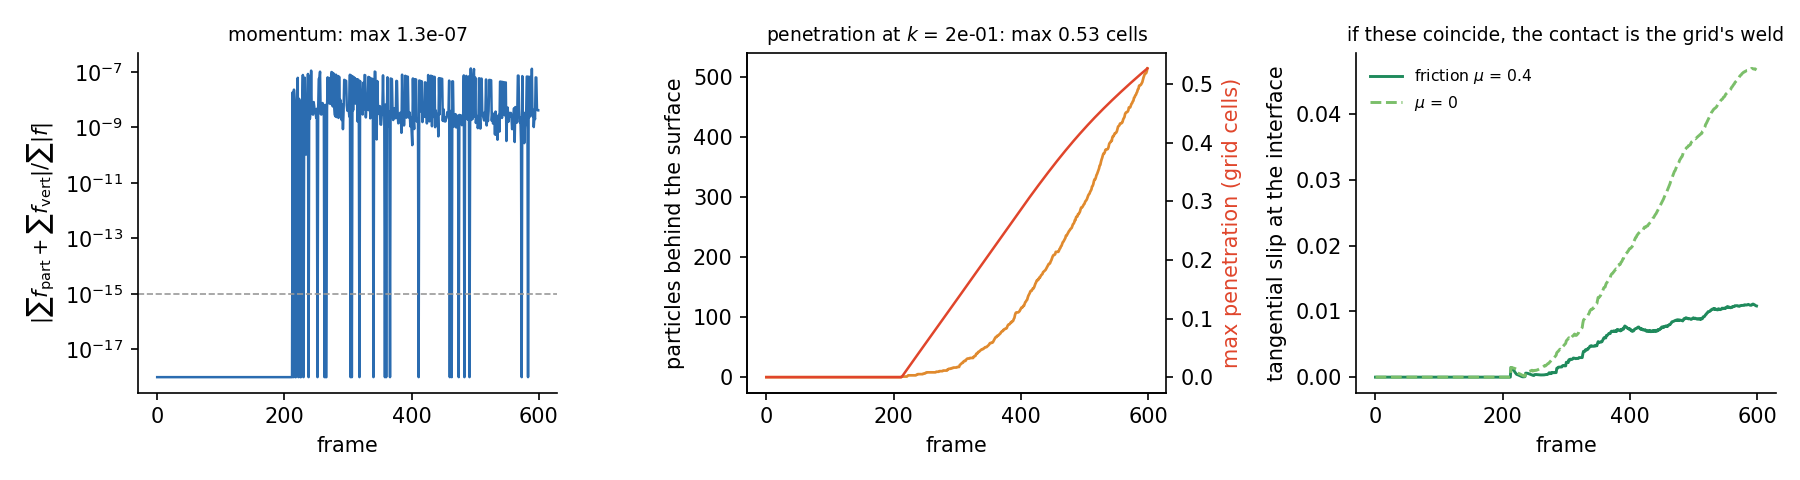
\includegraphics[width=\textwidth]{fig_mesh_contact_metrics.png}
\caption{Left: the momentum residual, which is the test that a one-way coupling fails by construction.
Middle: how many particles are behind the surface and how deep, in grid cells. Right: tangential slip
with friction and without --- if these two coincided, the ``contact'' would be MPM's automatic weld
wearing a friction coefficient.}
\end{figure}

\textbf{Two failures the rig produced before it produced a result}, both worth keeping. Under gravity
the block \emph{fell out from under the patch} --- its floor is twenty cells below its underside, so it
was in free fall and the two bodies never met (block top $0.5800\to0.5728$ while the patch went
$0.5850\to0.5778$). And a patch of independent vertices is not a mesh: pressing its rim left the
interior behind, so the lattice needed edge springs before a press could load anything.

\section*{5.\; What this does and does not license}

It licenses the interface: a surface and a continuum can exchange force conservatively at a resolution
where grid-node coupling cannot, with slip that is a material property rather than a numerical
accident. It does not license the geometry --- the patch is flat and axis-aligned, so face lookup is
$O(1)$ and a real mesh needs a BVH --- and it does not license the accuracy: half a grid cell of
penetration is a lot, and the fix is either a stiffer penalty with a smaller substep or the barrier
formulation (BFEMP, Li et al.\ 2022), which forbids penetration outright at the cost of an implicit
solve. The next question is whether the same operator survives a \emph{curved, moving} mesh, which is
the spheroid.

\end{document}
